\chapter{THIS THESIS IN BRIEF}

This chapter explains the essential components of the three experiments that make up the majority of this thesis work: First, a measurement of the static polarizabilities of sodium, potassium, and rubidium (section \ref{polBrief}). Next, a novel and more precise method to measure the velocity of atom beams (section \ref{choppersBrief}) that will improve future polarizability measurements. Then, a measurement of a wavelength of light at which the dynamic polarizability of potassium is zero, known as magic-zero wavelength (section \ref{mzwBrief}). This chapter also contains summaries of a proposal to measure the polarizability of strontium using a photoionization detector, and a proposal to measure the tensor polarizabilities of alkali dimers.



%%%%%%%%%%%%%%%%%%%%%%%%%%%%%%%%%%%
\pagebreak
\section{Static polarizability measurements of Na, K, and Rb}
\label{polBrief}

In 2008, we set out to establish a new atomic polarizability measurement program in Arizona. In 2010 we published the first improved measurements of potassium and rubidium polarizability in over 35 years \cite{Hol10}. The paper, published in \emph{Physical Review A}, is included in Appendix \ref{polPRAappendix}. Chapter \ref{polChapter} explains additional details of this experiment. Section \ref{introPolHistory} reviewed the history of polarizability measurements and Figure \ref{polPreviousWorkPlot} summarizes previous calculations and measurements of alkali polarizabilities.

We measured the polarizabilities of sodium, potassium, and rubidium using a Mach-Zehnder atom interferometer with an interaction region containing an electric-field gradient. The interferometer and electrodes are shown in Figures \ref{ifm2010pra} and \ref{int2010photo}. We measured each polarizability (for Na, K, and Rb) independently, and we refer to these as absolute measurements. We also reported ratios of polarizabilities, since we can do this with even higher precision. Table \ref{polResultsTable} shows the absolute measurements (less than 1.0\% uncertainty), and Table \ref{polRatiosTable} shows the ratio measurements (0.3\% precision). 

Our measurements of polarizability ratios are new in atom interferometry, and are possible because nanogratings diffract all types of atoms and molecules. Although this unique feature of our interferometer has long been recognized, the work described in this thesis is the first time that the utility of nanogratings for multiple species has actually been used for a precision measurement of polarizability. The benefit of presenting ratios is that systematic errors are nearly the same for different atomic species and cancel when determining polarizability ratios. We combined our ratio measurements with the higher-precision measurement of sodium polarizability by Ekstrom \etal \cite{Eks95} to present the most precise measurements of potassium and rubidium polarizability currently available. Our measurements were recently included in an updated table of polarizabilities in the CRC Handbook of Chemistry and Physics \cite{Mil12}.


\begin{figure}
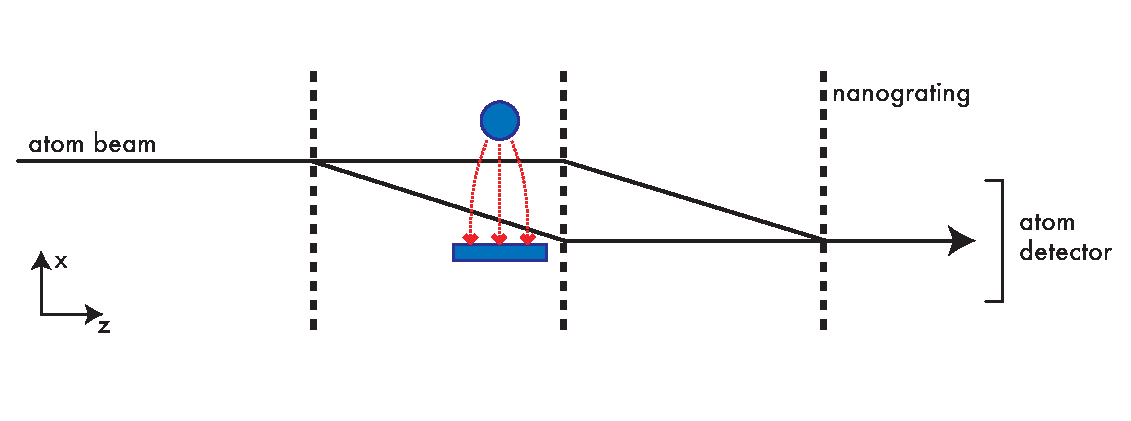
\includegraphics[width=1\textwidth]{Figures/ifmWith2010pol.eps}
\caption[Interferometer with polarizability measurement electrodes.]{\label{ifm2010pra} Atom interferometer with electric field gradient region (blue electrodes, red field lines) to measure static polarizabilities. An atom passing through the interaction region acquires a phase shift along each path and we measure the differential phase shift.}
\end{figure}


\begin{figure}
\centerline{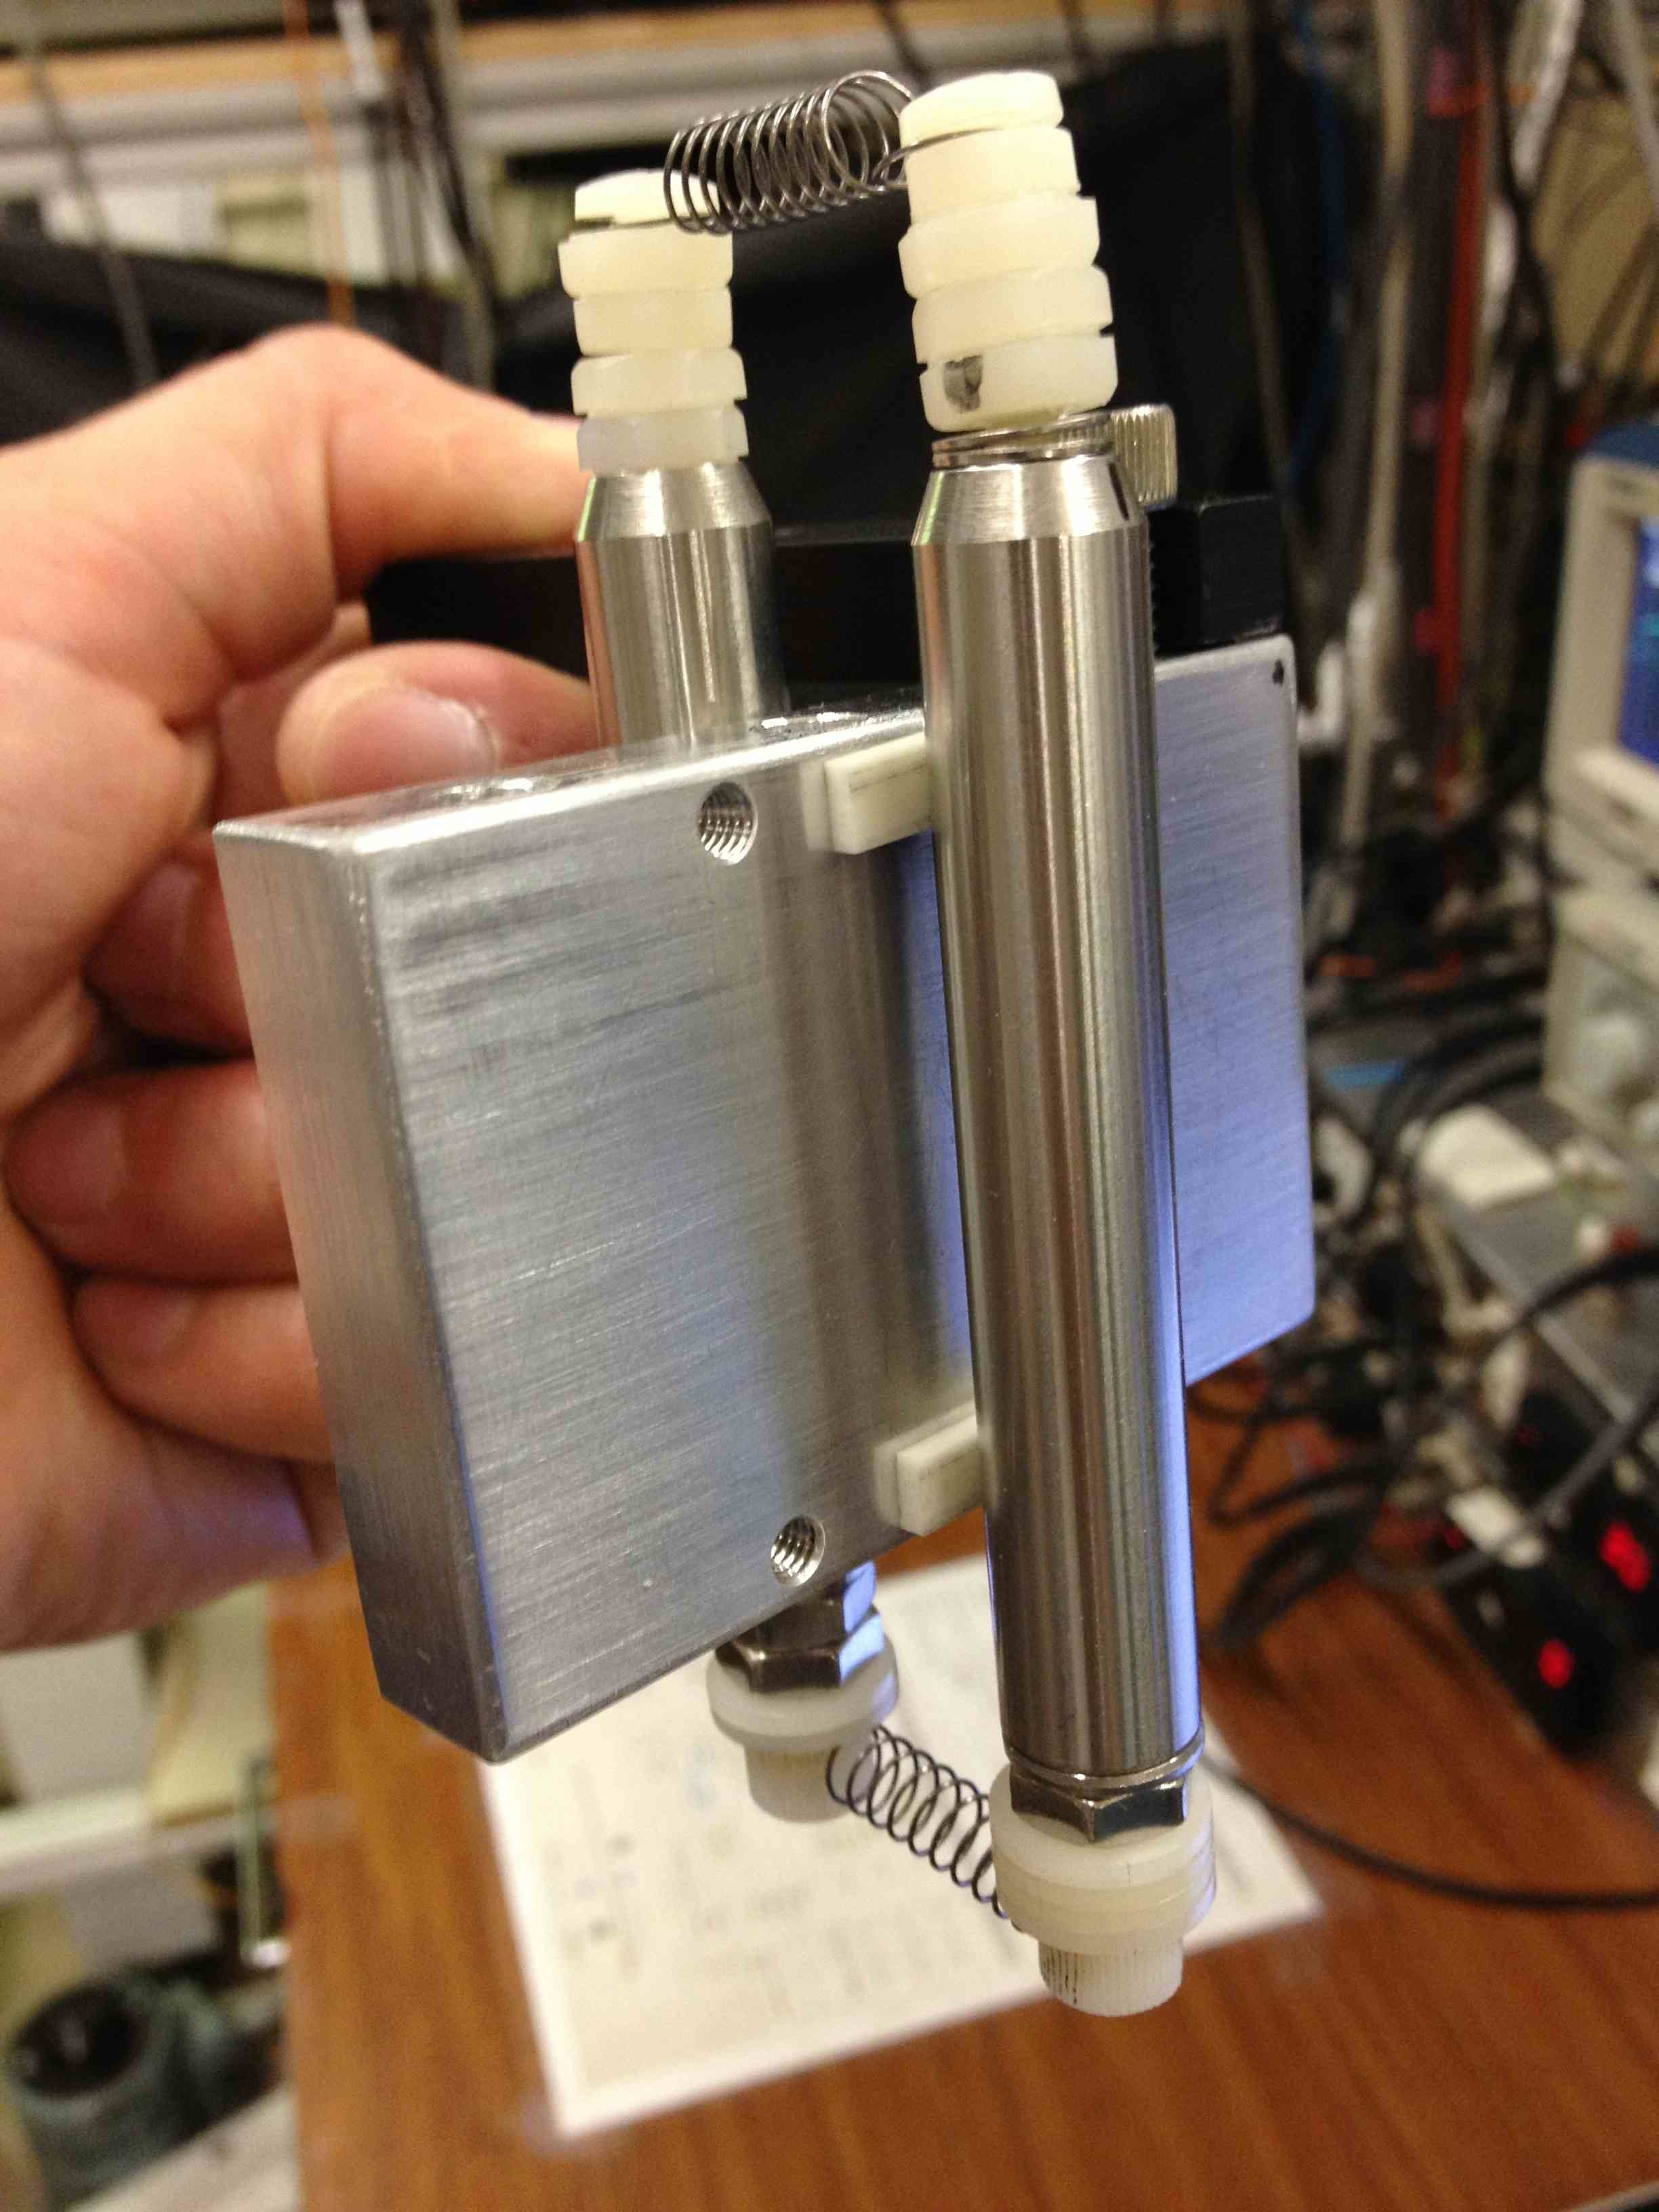
\includegraphics[width=.40\textwidth]{Figures/intRegion2010photoCompMore.jpg}}
\caption[Photograph of the 2010 polarizability measurement electrodes.]{\label{int2010photo}Photograph of the polarizability measurement electrodes. The atom interferometer paths pass through electric-field gradient between the rectangular ground plane and the cylindrical electrode.}
\end{figure}


\begin{table}
\caption[2010 PRA measurements of atomic polarizabilities.]{\label{polResultsTable}Measured absolute and recommended atomic polarizabilities in units of $10^{-24}\textrm{ cm}^3$.  Our recommended polarizability values are based on our ratio measurements (see Table \ref{polRatiosTable}) combined with the sodium polarizability measurement from Ekstrom \etal \cite{Eks95}.}
\begin{center}
\begin{tabular}{c c c c}
\hline\hline
& $\alpha_\textrm{abs}$(stat.)(sys.)  & { $\textrm{  }$ $\textrm{  }$ } & $\alpha_{\textrm{rec}}$(tot.)\\
\hline
Na & 24.11(2)(18) & & 24.11(8)\\
K & 43.06(14)(33) & & 43.06(21)\\
Rb & 47.24(12)(42) &  & 47.24(21)\\
\hline
\end{tabular}
\end{center}
\end{table}



\begin{table}
\caption[2010 PRA measurements of atomic polarizability ratios.]{\label{polRatiosTable}Measured atomic polarizability ratios with statistical uncertainties. Also included are several polarizability ratios from \emph{ab initio} and semi-empirical calculations. See Fig.~\ref{polPreviousWorkPlot} for more calculations and measurements of polarizability ratios.}
\begin{center}
\begin{tabular}{c | c | c c c}
\hline\hline
 &  $\alpha_\textrm{ratio}$(stat.~unc.) & & Theory\\
Atoms & This work & Ref \cite{Der99} & Ref \cite{Saf99} & Ref \cite{Mit03} \\
\hline
Rb/Na & 1.959(5) & 1.959(5) & 1.946 & 1.939 \\
K/Na    & 1.786(6) & 1.785(6) & 1.779 & 1.781 \\
Rb/K    & 1.097(5) & 1.098(5) & 1.094 & 1.089 \\
\hline\hline
\end{tabular}
\end{center}
\end{table}



\begin{figure}
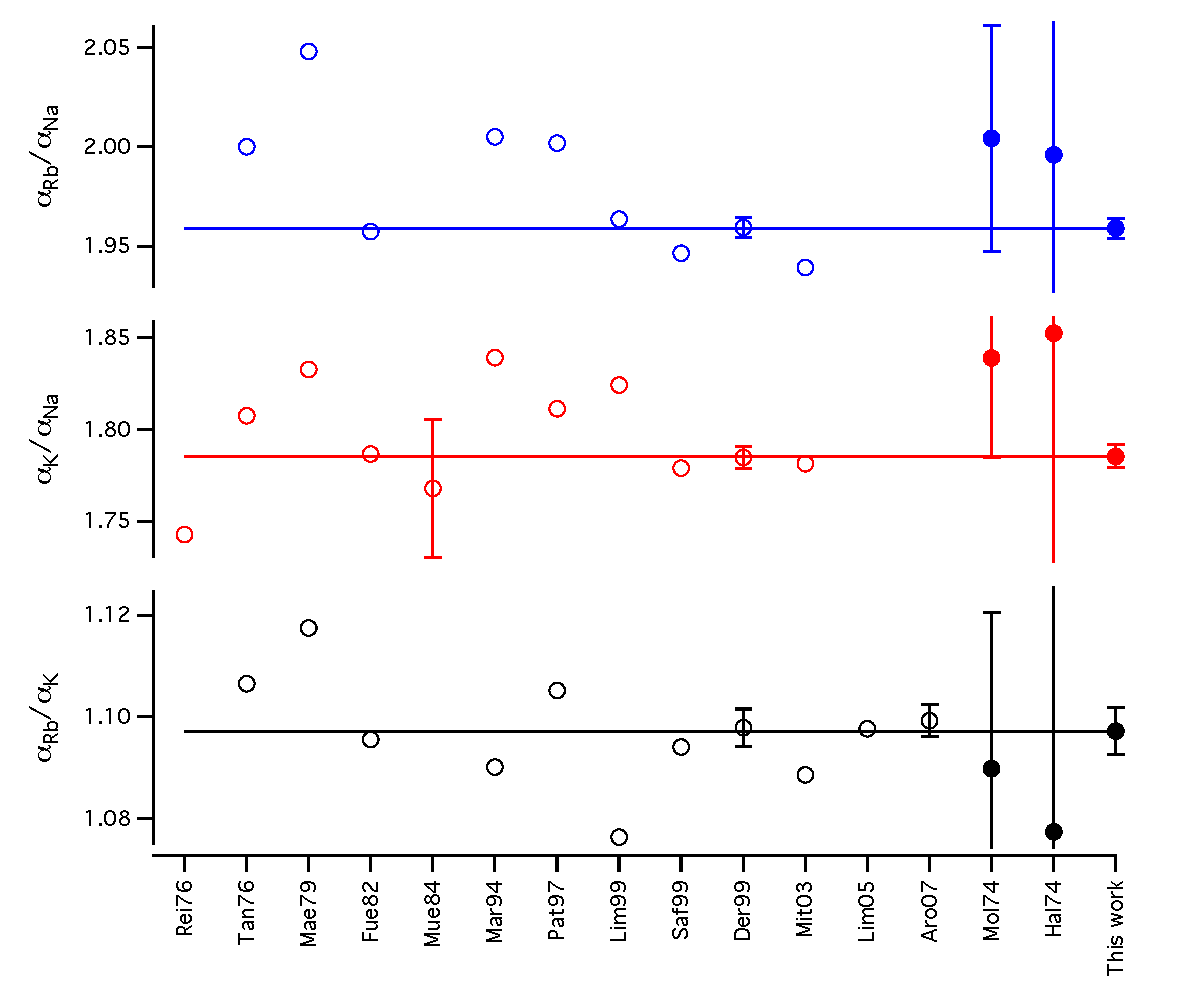
\includegraphics[width=1\textwidth]{Figures/PolPRAratios.pdf}
\caption[Previously calculated and measured alkali polarizability ratios.]{\label{polPreviousWorkPlot} Previously calculated (unfilled) and measured (filled) alkali polarizability ratios. References are denoted by the abbreviated first author's name and the publication year. Calculations in references Derevianko \etal (1999) \cite{Der99} and Arora \etal (2007) \cite{Aro07} incorporate state lifetime measurements.}
\end{figure}



Another unique feature of this work compared to other atom interferometry measurements of polarizability \cite{Eks95,Mif06} is that we use an electric-field gradient region to apply phase shifts to both paths rather than a septum electrode, which would apply a phase shift to only one path. Electric-field gradient regions have the advantage of not requiring an electrode to be placed between the two atom beam paths. This allows us to study heavier atoms with shorter de Broglie wavelengths and therefore smaller path separations. Since the electric-field gradient interaction region does not require resolved diffraction orders, another advantage is that we can use a less collimated beam to increase the flux and reduce the systematic error caused by velocity-selective detection of atoms in the interferometer. However, electric-field gradient regions have the disadvantage that the measured differential phase shift is proportional to $1/v^2$, rather than $1/v$, so the uncertainty in beam velocity measurements contributes twice as much to uncertainty in polarizability measurements. The phase shift in an electric-field gradient region also depends sensitively on the location of the atom beam paths with respect to the electrodes, unlike in a septum geometry with a uniform electric field. 


\begin{figure}
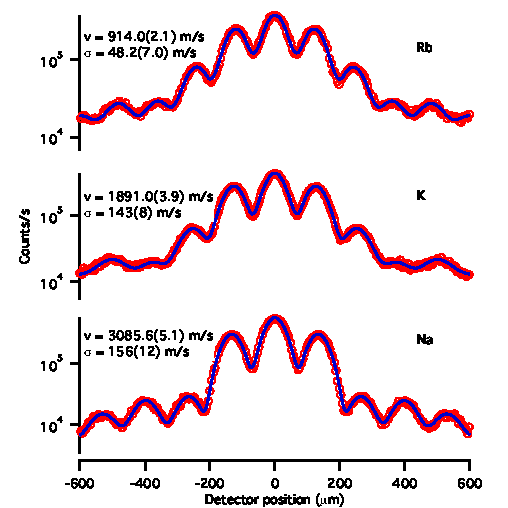
\includegraphics[width=1\textwidth]{Figures/Fig3Diffraction2.pdf}
\caption[Diffraction of Na, K, and Rb.]{\label{nakrbDiffraction} Diffraction of Na, K, and Rb atoms determines the average velocity, $v_0$, and the velocity distribution width, $\sigma_v$, of the atom beams. Figure \ref{diffractionPofv} shows the velocity distributions determined by these measurements.}
\end{figure}



The primary limitation of the absolute polarizability measurements in this experiment was determining the velocity and velocity distribution of the atom beam. We determined the atom beam velocity by studying atomic diffraction patterns in the far-field of the first nanograting, such as those shown in Figure \ref{nakrbDiffraction}. The atom beam velocity is given by rewriting equation \ref{sepEqn} as
\begin{eqnarray}
v(x_n)=\frac{z_{det}hn}{md_gx_n}
\end{eqnarray}
where $z_{det}$ is the distance from the first nanograting to the detector, and $x_n$ is the position of the $n$th diffraction order. In reality, a distribution of velocities exists in the supersonic atom beam, and this leads to a distribution of diffraction patterns. The velocity distribution can be well described by a Gaussian with an average velocity $v_0$ and width $\sigma_v$. Figure \ref{diffractionPofv} shows examples of typical supersonic atom beam velocity distributions. To better compare velocity distributions with different average velocities, it is useful to define a sharpness ratio $r=v_0/\sigma_v$. 




Each observed diffraction pattern is a convolution of the atom beam profile, the detector width, and the atom beam velocity distribution. Figure \ref{diffractionConv} illustrates the individual features that lead to the observed diffraction patterns. Uncertainties in $z_{det}$, the detector translation angle, and the details of this convolution limited the accuracy of the velocity measurement to 0.3\%, and thus contributed 0.6\% uncertainty to the absolute polarizability measurements. 


\begin{figure}
\centerline{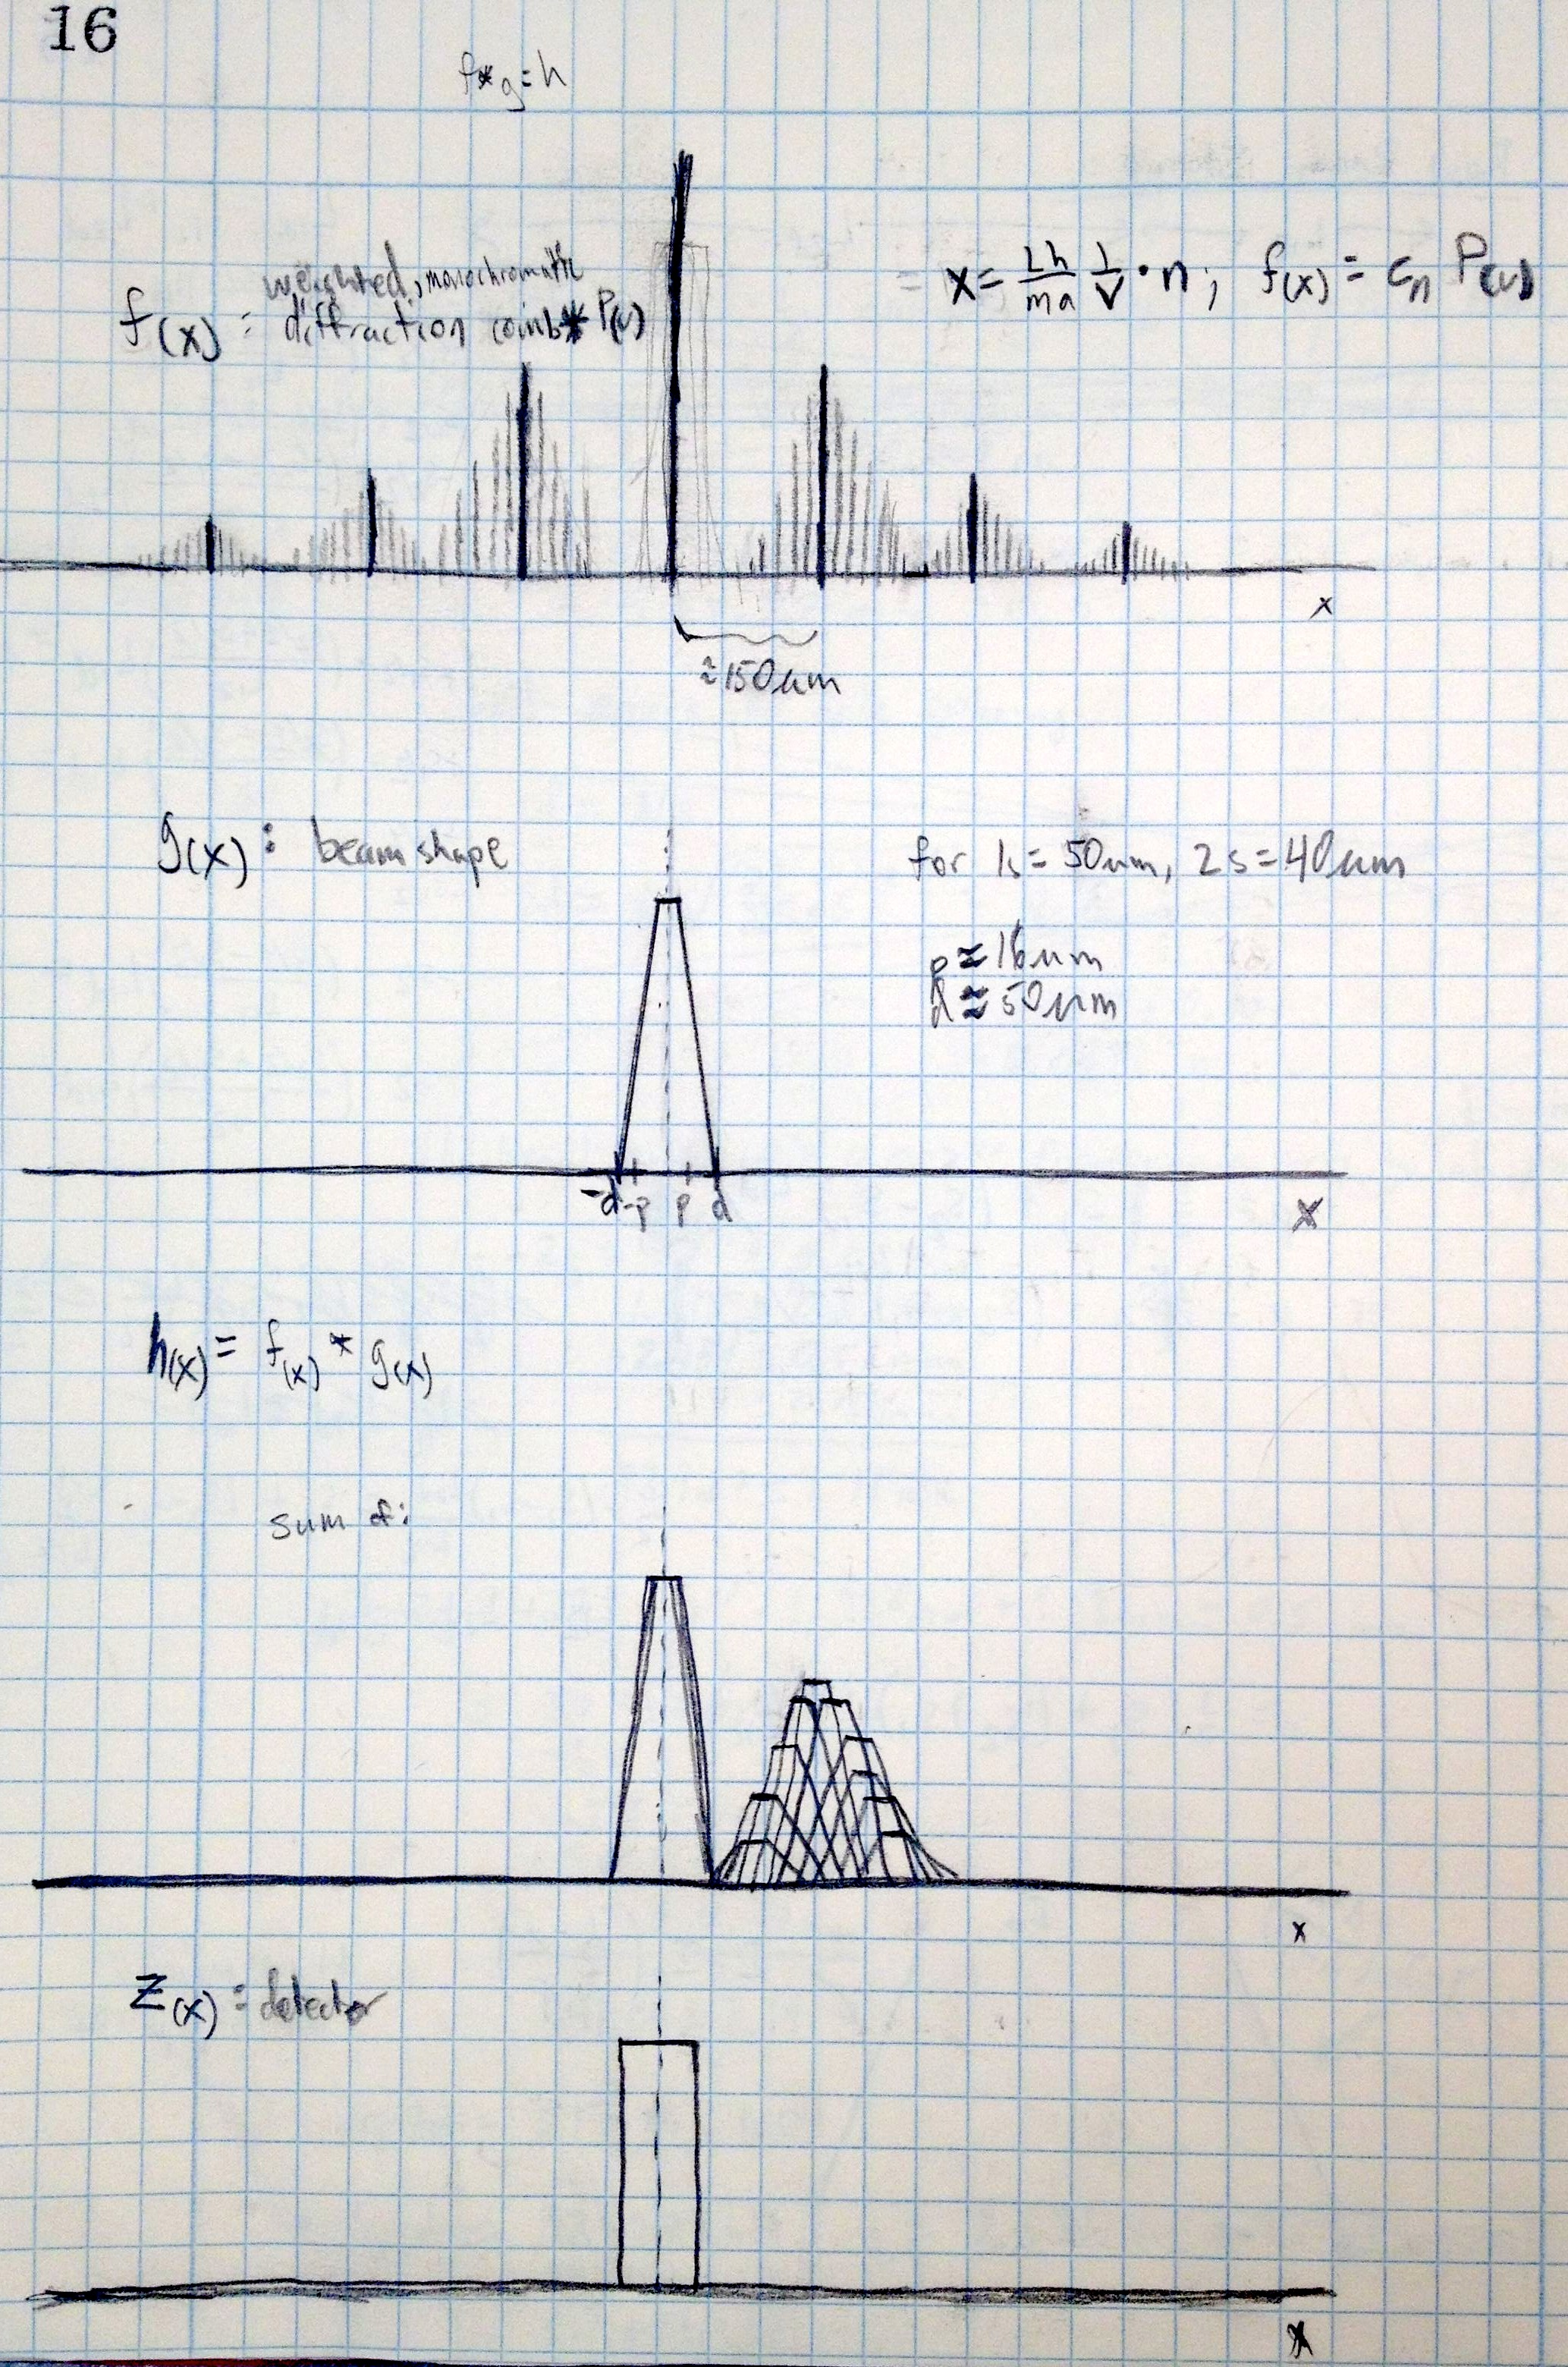
\includegraphics[width=.75\textwidth]{Figures/diffractionConvolution4.jpg}}
\caption[Convolution of atom beam profile, detector width, and velocity distribution for diffraction patterns.]{\label{diffractionConv} From top to bottom the plots show: the diffraction comb for different velocity classes, the trapezoidal atom beam profile obtained using two collimating slits, the convolution of the beam profile with the velocity distribution, and the hot-wire detector size. Figure from Will Holmgren lab notebook number 1 (June 2008).}
\end{figure}



If we ignore smaller effects such as the velocity distribution and the atom beam thickness (treated in detail in Appendix A), we can obtain a simple expression for the measured polarizability:
\begin{eqnarray}
\label{simplePol}
\alpha \approx \frac{v^2}{kV^2x_\textrm{int}}\phi_\alpha.
\end{eqnarray}
Here, $k$ is a constant that depends on the geometry of the interaction region, $V$ is the voltage applied to the interaction region, and $x_\textrm{int}$ is the transverse position of the interaction region. Figure \ref{phasePosition2010} shows a plot of the phase shift as a function of the interaction region position.

\begin{figure}
\centerline{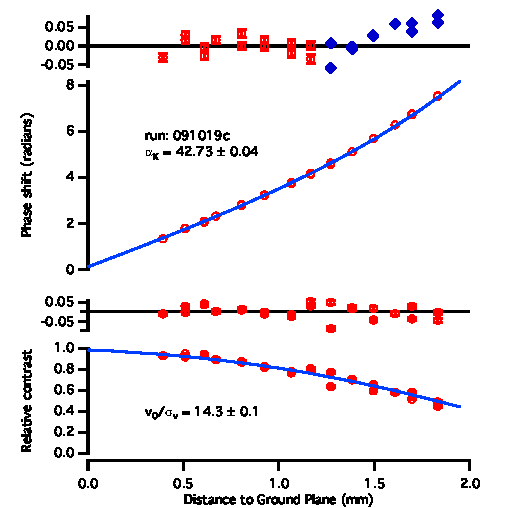
\includegraphics[width=0.75\textwidth]{Figures/Fig4PhaseFit.pdf}}
\caption[Phase shift and contrast vs.~interaction region position.]{\label{phasePosition2010} Interferometer phase shift and relative contrast vs.~interaction region position. We fit the phase shift data to determine the atomic polarizability. Higher phase shift data (blue points) was excluded from the fit due to their higher sensitivity to uncertainties in the velocity distribution width.}
\end{figure}

To measure the atom beam position $x_\textrm{int}$, we blocked the atom beam with the high voltage electrode and then moved the electrodes until the atom beam was visible again. Analysis of the transmitted flux vs.~electrode position allowed us to determine the atom beam position with a precision of 1 $\mu$m. We refer to this as the eclipse method. Unfortunately, we later determined that the motor position report was not as reliable as desired, and contributed a random error to the polarizability measurements. For the electrodes used in this experiment, a 10 $\mu$m error in beam position caused a 1\% error in the polarizability measurement. We now believe that 5-10 $\mu$m position errors were likely for each of the phase measurements, and this led to additional random error in the polarizability measurements. See section \ref{polChapterGradElg} for more details.


All systematic sources of error, such as uncertainty in $z_{det}$, the interaction region geometry, or the electrode voltages, are nearly identical for each atomic species. At the level of precision of our experiment, these systematic uncertainties cancel when presenting ratio measurements of polarizabilities. We measured the polarizability of each atomic species between 13 and 23 times (see Figure \ref{polPRAmeasurementsTrim}) and the reproducibility of the measurements determines the statistical uncertainty. The reported statistical uncertainty is the standard error of the mean. The irreproducibility of the data was larger than we expected given the interferometer contrast and count rate, primarily due to the faulty electrode position measurements.  


To improve upon our 2010 polarizability measurements, we developed a next-generation static polarizability experiment to reduce most uncertainties associated with this experiment. We developed a new velocity measurement technique (described in the next section), changed the geometry of the electric-field gradient region, improved the electrode position measurement, improved a number of distance measurements, and developed a new data acquisition system. Sections \ref{newDAQ} and \ref{polChapterGradElg} and Chapter \ref{choppersChapter} discuss the improved system in more detail.





%%%%%%%%%%%%%%%%%%%%%%%%%%%%%%%%%%%%%%%
\pagebreak
\section{Phase choppers: a new atom beam velocity measurement technique}
\label{choppersBrief}

Atom beam velocity was the largest source of uncertainty in our 2010 polarizability measurements. To reduce this uncertainty we developed a new technique to measure atom beam velocity called \emph{phase choppers} \cite{Hol11}. Phase choppers provide a more precise and more accurate measurement of beam velocity than can be obtained with diffraction. Chapter \ref{choppersChapter}, Appendix \ref{choppersAppendix}, and C.E. Klauss' B.S.~thesis \cite{Kla11} describe this technique in detail. Phase choppers are similar to the phase shifters described in \cite{Rob04} and their utility for measuring beam velocity was first proposed in \cite{Rob02}. Here, we summarize the most important features.

Phase choppers have numerous advantages over atom beam diffraction and other velocity measurement techniques:
\begin{enumerate}
\item Higher precision measurements in less time
\item Frequency-based instead of length-based measurement
\item No need for well-separated diffraction orders, so choppers can be used with faster beams (higher flux) and more massive atomic species
\item \emph{in situ} measurement of velocity distribution of atoms contributing to the interference fringes
\item No moving parts
\end{enumerate}

To understand how phase choppers can measure atom beam velocity, it helps to first consider mechanical choppers. Two spinning mechanical choppers (slotted disks) separated by a distance $L$ and blocking the beam at frequency $f$ can transmit atoms with velocity $v = nLf$, where $n$ is an integer. An atom with velocity $v$ will travel a distance $L$ from the first chopper to the second chopper in a time $\tau=L/v$, corresponding to a fundamental chopping frequency $f_0=v/L$. 

Mechanical choppers simply block or transmit atoms, leading to a maximum in the transmitted flux when the chopping frequency is any integer multiple of $f_0$. In the method we present here, phase choppers are switched on and off by a function generator to periodically apply phase shifts to atomic de Broglie waves in an interferometer. This leads to a maximum in the interferometer \emph{contrast}, instead of the \emph{flux}, when the chopping frequency satisfies $f=n f_0$. The ability to control wavefunction phase, rather than amplitude, provides a more featured and higher flux data set and allows for a more precise determination of velocity. 


\begin{figure}
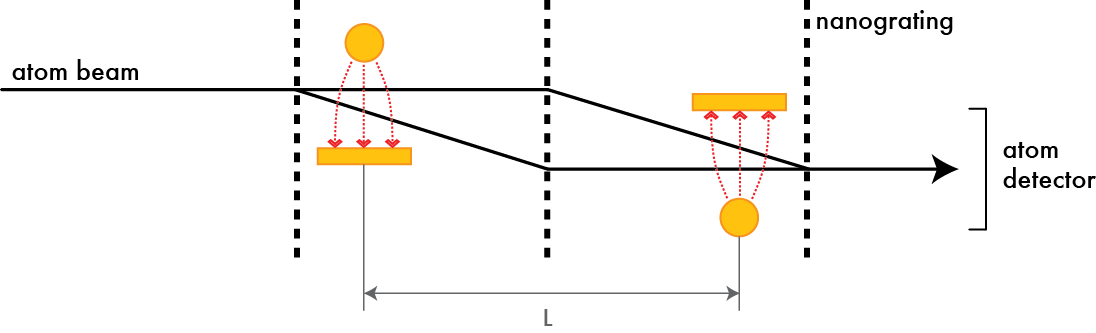
\includegraphics[width=1\textwidth]{Figures/IFMwithChoppers.png}
\caption[Phase choppers in the atom interferometer.]{\label{choppersIFMsimple}Two phase choppers are placed in the interferometer at a distance $L = 1270.68(25)$ mm apart. A square-wave voltage $V(t)$ applied across the choppers creates an electric field (dashed lines). Atoms with velocity $v$ passing through chopper 1 and chopper 2 acquire net differential phase shifts $\phi_1(t)+\phi_2(t+L/v)$.}
\end{figure}


Figure \ref{choppersIFMsimple} shows two phase choppers added to the atom interferometer. Before continuing, it is worth restating an important principle regarding how our atom interferometer works: the observed fringe pattern is the incoherent sum of the sinusoidal probability distributions from single-atom interference, repeated about $10^5$ times per second. Different atoms have different velocities and enter and exit the interferometer at different times. We observe an ``average" of all of these fringe patterns. Therefore, if half of the atoms receive phase shifts that are $\pi$ different from the other half of the atoms, then the measured interference contrast $C$ will be 0. Mathematically, we would observe an intensity $I=I_0 + C_0(0.5\sin(k_x x)+0.5\sin(k_x x+\pi))=I_0+C\sin(k_x x)$ with $C=0$. 

\begin{figure}
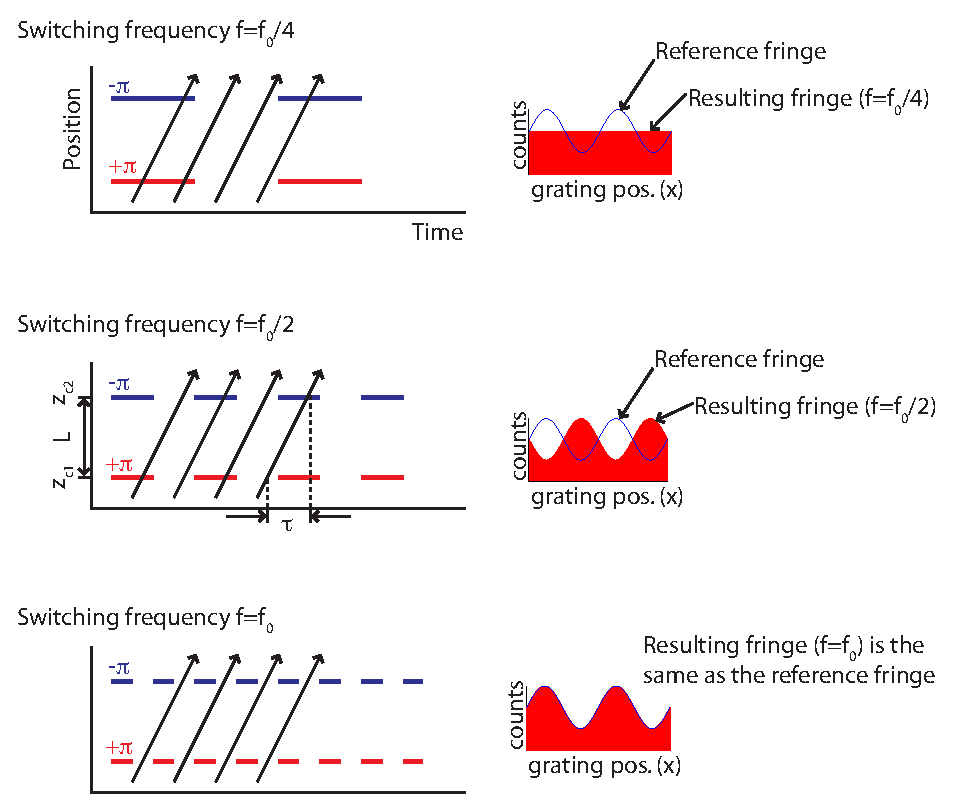
\includegraphics[width=1\textwidth]{Figures/PhaseChoppersVvst4.eps}
\caption[Interferometer contrast for particular chopping frequencies.]{\label{VvsT}Atoms with different starting times will acquire 0, $+\pi$ (red), or $-\pi$ (blue) phase shifts as they pass through chopper 1 and chopper 2, depending on their velocity $v$ and the chopping frequency $f$. The time it takes an atom with velocity $v$ to travel the distance $L$ between the choppers is $\tau$ and $f_0=1/\tau$. We measure the average of the sinusoidal probability distributions formed by each atom interfering with itself, shown at right. The reference interference pattern with the choppers off is shown in blue and the resulting interference patterns with the choppers on are shown in red.}
\end{figure}

Depending on its start time, velocity, and the chopping frequency, an atom will pass through the two choppers in one of four possible pairs of conditions (off-off, on-off, off-on, or on-on). We now describe what happens to the interference pattern created by atoms with a single velocity $v$ when the choppers are switched at four particular frequencies (see Figure \ref{VvsT}):
\begin{itemize}
\item $\bm{f \ll f}\bm{_0}.$ Atoms experience the off-off (0 net differential phase shift) or on-on (0 net differential phase shift) pairs of conditions with equal likelihood, and all atoms emerge with 0 net phase shift. The contrast and phase of the detected ensemble remain unchanged.

\item $\bm{f=f}\bm{_0/4}$. Atoms experience each of the four possible pairs of conditions, off-off (0), on-off ($\pi$), off-on (-$\pi$), or on-on (0), with equal likelihood. Therefore, half of the ensemble will acquire 0 net differential phase shift, and half will acquire a $\pi$ net differential phase shift. The ensemble contrast is 0 and phase is indeterminate. Contrast minima repeat at frequencies $f=(2n+1)f_0/4$, where $n$ is an integer. 

\item $\bm{f=f}\bm{_0/2}$. Atoms experience on-off ($\pi$) or off-on ($-\pi$) pairs of conditions with equal likelihood. The ensemble contrast remains unchanged, but the phase shifts by $\pi$ (modulo $2\pi$). Contrast revivals with $\pi$ phase shifts repeat at frequencies $f=(2n+1)f_0/2$. 

\item $\bm{f=f}\bm{_0}$. Once again, all atoms experience the off-off (0) or on-on (0) states. The ensemble contrast and phase remain unchanged. Contrast revivals with no phase shift repeat at frequencies $f=nf_0$.
\end{itemize}

These simple cases show how by finding the value of $f_0$ one can find the velocity of an atom beam through the relation $v=Lf_0$. The contrast revivals and minima that occur at large $n$ provide a way of leveraging small changes in velocity into large changes in revival and minima frequency. In practice, we find the velocity of our atom beam by measuring the contrast at many frequencies and fitting the contrast data to a model discussed in Appendix B. Figure \ref{CsSimpleChopperScan} shows fitted data from a typical chopper frequency scan using this model. The major corrections to the simple model include methods to account for velocity distribution, velocity dependent phase shifts from the choppers, application of non-$\pi$ average phase shifts, and velocity-dependent phase shifts due to the Sagnac effect.


\begin{figure}
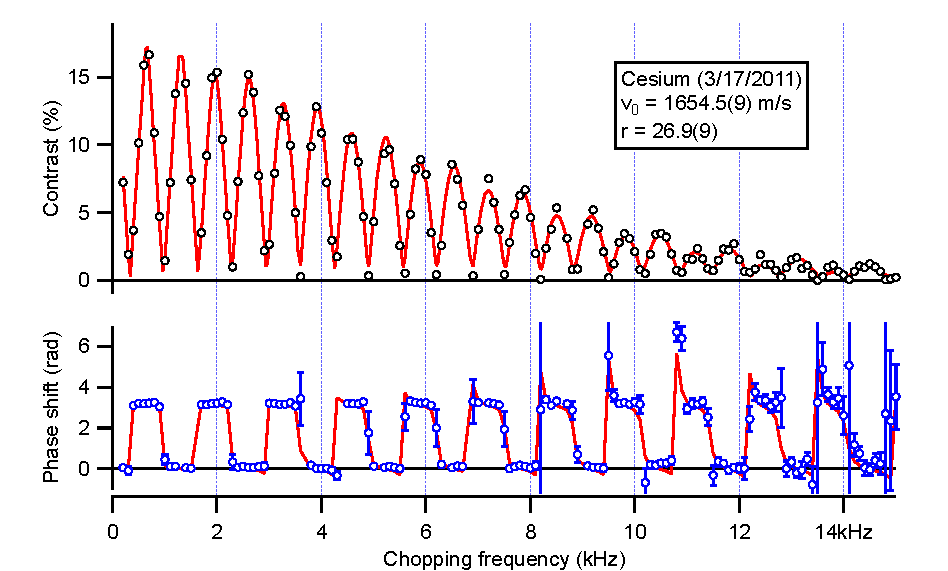
\includegraphics[width=1\textwidth]{Figures/CsSimpleChopperScan.pdf}
\caption[Phase chopper data and best-fit functions.]{\label{CsSimpleChopperScan}Phase chopper data (circles) and corresponding best-fit functions (red curves) for a cesium atom beam with a 70\% helium, 30\% argon carrier gas. We fit the contrast (black) to find the flow velocity $v_0$ and velocity ratio $r=v_0/\sigma_v$. The measured phase (blue) is also shown, but is not fit. Each point is derived from 5 seconds of data. Note that the asymmetric slope of the phase data is due to the Coriolis deflection (Sagnac phase shift).}
\end{figure} 


We also tested the phase choppers by measuring the polarizability of cesium using beams with three very different flow velocities on three different days. Each day we alternated between measurements of beam velocity and polarizability every hour to account for small changes in velocity ($<0.5\%$) over the course of a day due to instability in the beam source temperature. The statistical error of each measurement of velocity was less than 0.1\%. We found the cesium polarizability (stat.~unc.) to be 59.84(4), 59.71(7) and 59.85(8) $\mathrm{\AA}^3$ at flow velocities of 925, 1345 and 1680 m/s. This data is shown in Figure \ref{csPolVelDiff}. These polarizability measurements are subject to a systematic correction due to a revised measurement of the interaction region geometry, but the consistency of the polarizability measurements provides strong evidence that our velocity measurements using phase choppers are reproducible at the 0.1\% level, similar to the measurement of Amini and Gould \cite{Ami03}.







%%%%%%%%%%%%%%%%%%%%%%%%%%%%%%%%%%%%%%%%%
\pagebreak
\section{Measurement of a magic-zero wavelength}
\label{mzwBrief}

Most measurements of static and dynamic polarizabilities are limited by uncertainty in the electric field strength and uncertainty in the time an atom interacts with the field. To avoid these limitations, we designed an experiment to measure the wavelength at which the dynamic polarizability of an atom goes to zero. This is known as the \emph{magic-zero wavelength}, or \emph{tune-out wavelength}. We published our measurement in \emph{Physical Review Letters} \cite{Hol12a} (Appendix \ref{mzwAppendix}) and Chapter \ref{mzwChapter} includes supporting material for this experiment.


A magic-zero wavelength ($\lambdaZero$) occurs between atomic resonances, where the light is red-detuned from one resonance and blue-detuned from another. Opposing contributions from these resonances produce a root in the dynamic polarizability at $\lambdaZero$ and so the energy shift of an atom vanishes at $\lambdaZero$. Figure \ref{KredBlueMZWfig} shows the dynamic polarizability in the vicinity of the four lowest energy transitions of potassium. Three magic-zero wavelengths occur between these four transitions.


Magic-zero wavelengths are understandable in terms of the Lorentz oscillator model of an atom. The equation of motion for an electron in the Lorentz oscillator model yields
\begin{eqnarray}
x(t)=-\frac{e}{m}\frac{1}{\omega_0^2-\omega^2-i\omega\gamma}E(t)
\end{eqnarray}
where $e$ is the electron charge, $m$ is the electron mass, $\omega_0$ is the resonance frequency of the atom, $\omega$ is the frequency of oscillation of the electric field $E(t)$, and $\gamma$ is the damping parameter. We can define a complex polarizability $\alpha(\omega)$ in terms of the dipole moment $p(t)$:
\begin{eqnarray}
p(t)=-ex(t)=\alpha(\omega) E(t)\\
\alpha(\omega)=\frac{e^2}{m}\frac{\omega_0^2-\omega^2+i\omega\gamma}{(\omega_0^2-\omega^2)^2+(\omega\gamma)^2}.
\end{eqnarray}
The real part of the complex polarizability gives the dispersion and the imaginary part corresponds to absorption of light. Magic-zero wavelengths occur far from resonance, where the absorption probability is low and $|\omega_0-\omega|\gg\gamma$, so we drop the imaginary component:
\begin{eqnarray}
\label{alphaOmegaSimEqn}
\alpha(\omega)=\frac{e^2}{m}\frac{1}{\omega_0^2-\omega^2}.
\end{eqnarray}
Like any harmonic oscillator, the motion of the electron becomes $\pi$ radians out of phase with the driving field as the frequency of the driving field passes through resonance, and thus the polarizability changes sign as well. Equation \ref{alphaOmegaSimEqn} clearly shows that the polarizability changes sign as the frequency $\omega$ of the driving field passes through resonance. 


\begin{figure}
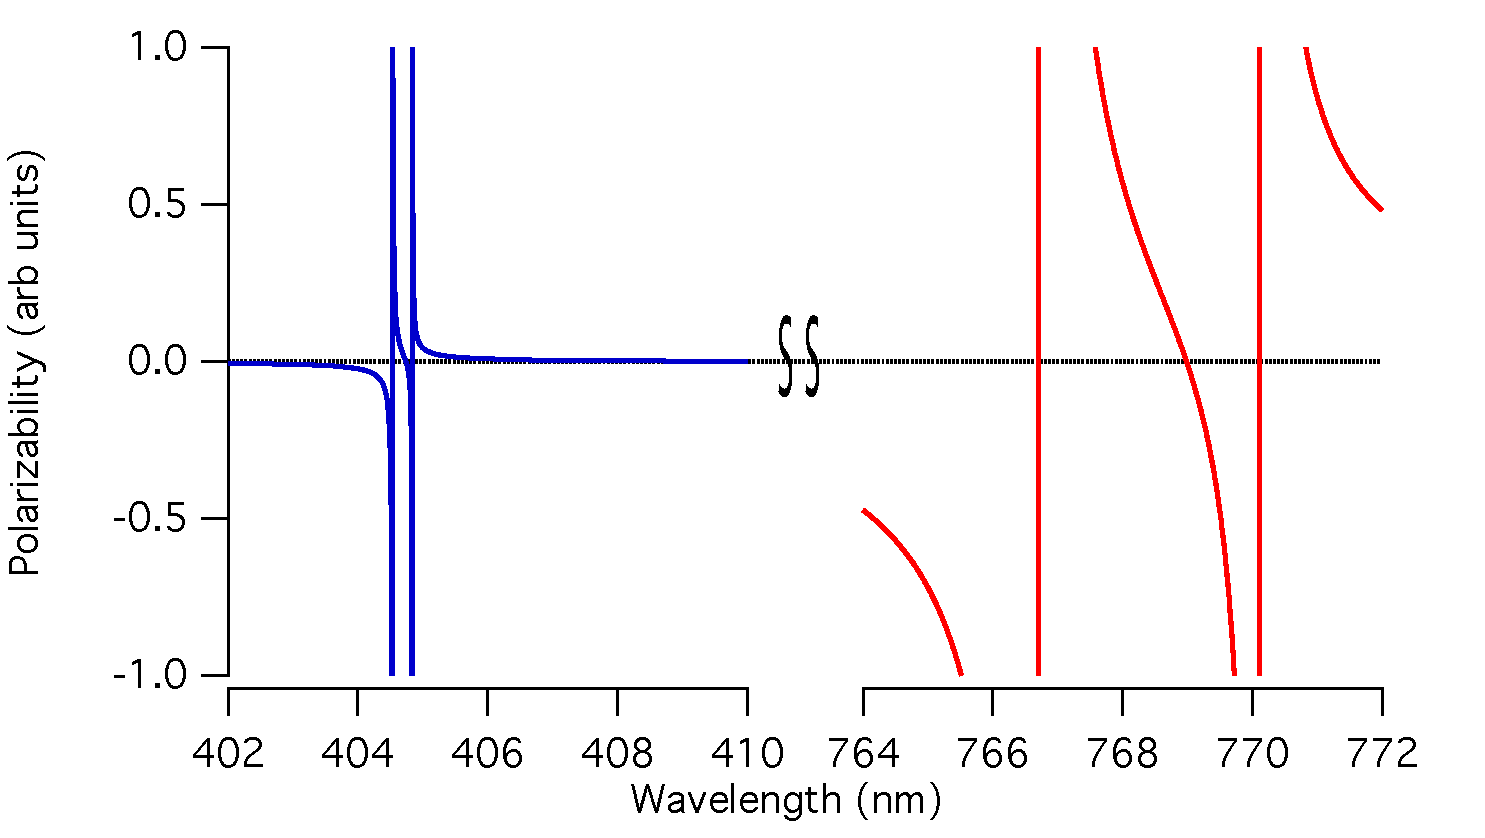
\includegraphics[width=1\textwidth]{Figures/KredBlueMZWedit.pdf}
\caption[Dynamic polarizability and magic-zero wavelengths of K.]{\label{KredBlueMZWfig}A plot of the dynamic polarizability of potassium in the vicinity of the $4s-4p$ (red) and $4s-5p$ (blue) transitions. Three zero-crossings, magic-zero wavelengths, are visible near 405 nm, 406 nm, and 769 nm. The blue and red transitions are shown using the same wavelength range to highlight the smaller fine structure splitting of the $4s-5p$ transitions.}
\end{figure}


Chapter \ref{mzwChapter} and Appendix \ref{mzwAppendix} describe in detail our measurement of the first magic-zero wavelength of potassium near 769.971 nm \cite{Hol12a}. This novel method to probe atom structure yielded the most precise determination of the ratio of the $D1$ to $D2$ line strengths. We found
\begin{eqnarray}
\label{Reqn}
R=\frac{S_2}{S_1}=\frac{|\langle 4s || D || 4p_{3/2}\rangle|^2}{|\langle 4s || D || 4p_{1/2}\rangle|^2}=2.0005(40).
\end{eqnarray}


Various $\lambda_\textrm{zero}$ have been used in experiments to study entropy exchange \cite{Cat09}, quantum information processing \cite{Dal08}, and diffraction of matter waves from an ultracold atom crystal \cite{Gad12}. We have also discussed future applications for magic-zero wavelengths such as measurements of hyperpolarizability, rotation sensing, additional line-strength measurements, and measurements of the contribution of core electrons to polarizabilities.


The longest magic-zero wavelengths for alkali atoms are determined mostly by the transition energies $\hbar\omega_1$ and $\hbar\omega_2$ and the ratio $R$ of the line strengths. We use the sum-over-states approach to describe the dynamic polarizability $\alpha(\omega)$ near these two transitions by
\begin{eqnarray}
\label{dynpol}
\alpha(\omega) = & \frac{1}{3\hbar} S_1 \left( \frac{\omega_1}{  \omega_{1}^2 - \omega^2} + R\frac{\omega_{2}} { \omega_{2}^2 - \omega^2} \right) + A
\end{eqnarray}
where $A$ accounts for contributions from core excitations, higher energy valence transitions, and core-valence coupling \cite{Saf06, Mit10}. At the longest magic-zero wavelength of potassium, $A$ is 0.02\% of the nearly equal and opposite contributions from the principal transitions to the polarizability and $A$ changes $\lambda_\textrm{zero}$ by 0.15(1) pm \cite{Saf12per}. Therefore, the theoretical uncertainty in this magic-zero wavelength calculation, 3 pm, is nearly entirely determined by uncertainty in the ratio of the line strengths, $R$. The total uncertainty of our $\lambdaZero$ measurement was 1.5 pm. 


To measure the magic-zero wavelength, we focused 500 mW of laser light asymmetrically on the paths of our interferometer. As stated previously, the energy shift of a polarizable atom is given by 
\begin{eqnarray}
U(\omega) = -\frac{1}{2} \alpha(\omega) \vec{E}^2(\omega,z,t)
\end{eqnarray}
where we now allow for a frequency dependence for the polarizability and the electric field. For optical frequencies, we can only measure the energy shift due to the time average of the electric field, i.e.~the intensity. The phase acquired along one interferometer path is given by $\alpha(\omega)$ and the intensity of the light $I(x,z)$ at that location:
\begin{eqnarray}
\label{mzwIntEqn}
\phi_0(\omega) = \frac{\alpha(\omega)}{2\epsilon_0 c \hbar v}\int_{-\infty}^{\infty}I(x,z) dz.
\end{eqnarray}
Similar to the static polarizability experiment, where we used a static electric field gradient, here, we use an intensity gradient to apply different phase shifts to each interferometer path. We measure the differential phase shift of the two interferometer paths. Measurements of these differential phase shifts as a function of optical frequency, or wavelength, allow us determine $\lambdaZero$.


The uncertainty of our $\lambdaZero$ measurement, 1.5 pm, was dominated by the reproducibility of the measurement. The statistical precision (2$\sigma$) of our experiment was 1.4 pm. Section \ref{mzwDataAnalysis} explains the relationship between the reproducibility and the data collection procedure in more detail. The broadband component of the light, shown in Figure \ref{ASEgratingPic}, was the largest source of systematic error (0.5 pm) in our measurement.


\begin{figure}
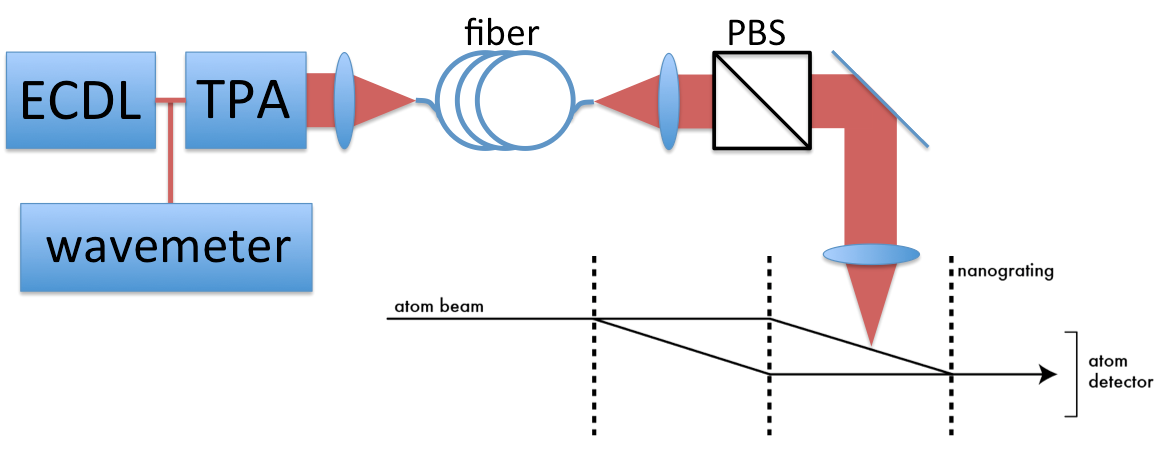
\includegraphics[width=1\textwidth]{Figures/mzwLaserSystem2.png}
\caption[Laser system for $\lambdaZero$ measurement.]{\label{mzwLaserSystem}Laser system for $\lambdaZero$ measurement. A grating-stabilized laser (ECDL) seeds a tapered amplifier (TPA). Light from the tapered amplifier is coupled into an optical fiber and then focused onto the atom interferometer. A wavelength meter measures the wavelength of the seed laser. Not shown is a shutter after the fiber to switch the light on and off, and an optical isolator on each side of the tapered amplifier.}
\end{figure}


%The laser spectrum is unfortunately not pure. Figure \ref{ASEgratingPic} shows the tapered amplifier light after being diffracted by a grating. Characterizing the laser spectrum is the leading contributor to the systematic uncertainty of our $\lambdaZero$ measurement.


\begin{figure}
\centerline{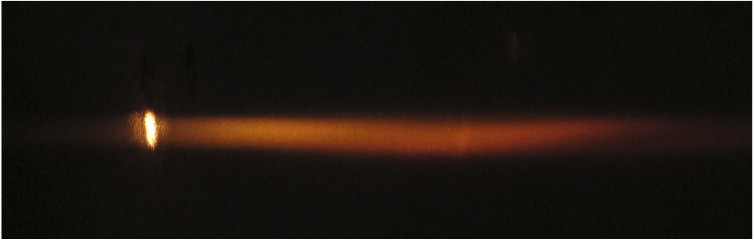
\includegraphics[width=.90\textwidth]{Figures/ASEpicture.png}}
\caption[Photograph of laser system spectrum.]{\label{ASEgratingPic}Photograph of the laser system spectrum. Light from the tapered amplifier was made to reflect off a diffraction grating and projected onto a screen. The spectrum shown spans approximately 50 nm. It is important to note that the photograph is a convolution of the frequency-dependent transfer function of the imaging system, including an infrared filter, with the spatially separated spectrum. Figure \ref{mzwSponData} shows the laser spectrum measured by a commercial grating spectrometer.}
\end{figure}


Interferometer contrast loss is primarily due to averaging over large distributions in phase shifts due to the atom beam velocity distribution and the nonuniform differential phase shifts across the atom beam. However, at the magic-zero wavelength we would naively expect zero phase shift for all atoms, and therefore no contrast loss. Unintended elliptical polarization of the laser beam combined with the unpolarized atom beam explains the contrast loss near $\lambdaZero$. Circular polarization causes different Zeeman substates ($m_F$) to acquire different phase shifts even at $\lambdaZero$. Section \ref{mzwContrast} explains the interferometer contrast loss in more detail.


This experiment can in principle be significantly improved before the photon scattering rate places a fundamental limit on the precision of a $\lambdaZero$ measurement. Let us imagine that we had unlimited laser power available and that we could focus all of the light on only one path of the atom interferometer to maximize the differential phase shift. Both the phase shift and the photon scattering rate grow in proportion to the laser power. However, the interferometer contrast, and thus the phase precision, decreases exponentially with the scattering rate. We therefore calculated a maximum achievable signal of 
\begin{eqnarray}
\label{TOWlimit}
\frac{d\phi}{d\omega}\approx\frac{1}{2\Gamma}P_\textrm{s}
\end{eqnarray}
where $P_\textrm{s}$ is the probability that an atom scatters one or more photons and $\Gamma$ is the excited state decay rate. With contrast loss due to scattering optimized to allow for maximum interferometric precision ($P_\textrm{s} = 1-e^{-1}$) the slope may become as large as $d \phi / d \lambda = $ 40 rad/pm. In this way, future measurements of magic-zero wavelengths can be made with very high precision, possibly with accuracy limited by a shot noise sensitivity better than picometers per $\sqrt{\textrm{Hz}}$. Section \ref{mzwLimitSection} contains a more detailed derivation of this limit.


Section \ref{mzwNextGenSec} discusses ideas to improve the precision of $\lambdaZero$ measurements in our lab. Improvements to the measurement precision would allow for benchmark tests of dipole matrix elements between the $ns$ and $(n+1)p$ levels in potassium and other alkali atoms. These matrix elements are more difficult to calculate due to larger relativistic corrections in the $(n+1)p$ levels. Interestingly, core electron contributions to polarizabilities may also be determined with $\lambdaZero$ measurements when combined with measurements of static polarizability and/or line strengths, depending on the particular atom and $\lambdaZero$. 







%%%%%%%%%%%%%%%%%%%%%%%%%%%%%%%%%%%%%%%%%
\pagebreak
\section{Strontium polarizability measurement proposal}
Polarizability measurements of strontium and ytterbium are currently highly desirable to support next-generation atomic clocks. The blackbody radiation environment surrounding atomic clocks changes the clock frequency by an amount proportional to the differential polarizability of the clock states and accurate polarizability measurements are required to calibrate this frequency shift. As an alkaline-earth atom with two valence electrons, strontium polarizability calculations are also more difficult due to electron correlations and call for experimental benchmarks. 


Unfortunately, our atom interferometer is currently unable to measure Sr polarizability due to low detection efficiency. Hot-wire detectors, like the one we use in our atom interferometer, do not ionize strontium atoms as efficiently as the alkali atoms. This is due to the ionization energy of strontium (5.7 eV) being larger than the work function of a platinum wire (5.5 eV). As a result, we presently can only detect collimated beams of strontium atoms in the absence of the nanogratings.


We propose that resonant photoionization can be used to provide high-efficiency and low-noise detection of strontium atoms. The photoionization pathway, shown in Figure \ref{srLevelsSimple}, involves absorption of a 461 nm photon to reach the $^1\textrm{P}_1$ state, and then absorption of a 405 nm photon to place the Sr atom in an autoionizing state. The existence of the autoionizing state increases the photoionization probability of Sr by a factor of about $10^3$.


\begin{figure}
\centerline{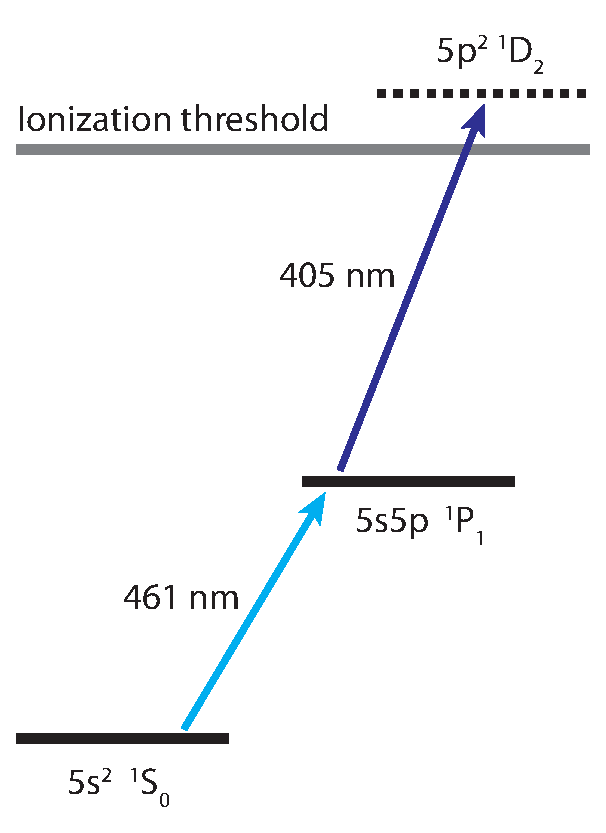
\includegraphics[width=.4\textwidth]{Figures/srLevelDiagramSimple.eps}}
\caption{\label{srLevelsSimple}Resonance enhanced photoionization pathway of strontium.}
\end{figure}


We propose a laser system consisting of a frequency doubled 922 nm laser diode and a free running 405 nm laser diode. A periodically poled KTP crystal can provide sufficient single pass frequency doubling efficiency (1-5\%), so we can avoid the complexity of a placing the crystal in a cavity. Generation of 1 mW of 461 nm light with less than 30 MHz linewidth and locked to the $^1\textrm{P}_1$ transition is the most difficult part of this proposed experiment. The 405 nm ionization laser can be relatively simple. The linewidth of the autoionizing transition is nearly 1 nm, so a high power 500 mW, multimode free running diode can be used.

Chapter \ref{alphaSrChapter} describes this proposal in more detail and is the topic of current research in our lab.






%%%%%%%%%%%%%%%%%%%%%%%%%%%%%%%%%%%%%%%%%
\pagebreak
\section{Tensor polarizability measurement proposal}

Ground-state alkali atoms are spherically symmetric, and as a result the polarizability may be described by a scalar that does not depend on the direction of the applied field. In contrast, molecules are generally not spherically symmetric and their polarizabilities must be described by a tensor $\tensorPol$. For a simple molecule such as an alkali dimer, the tensor is diagonal if one chooses to use the obvious axes of symmetry: one along the bonding axis of the molecule and two additional axes that are mutually orthogonal to the bonding axis. Figure \ref{dimerOrientationFig} shows the two unique orientations of an alkali dimer in an electric field. To our knowledge, only the average polarizability of this tensor has been measured \cite{Tar93,Mol74} for alkali dimers. Chapter \ref{dimersChapter} describes a proposal to measure the anisotropy of alkali dimer polarizability by studying contrast loss and revivals as a function of electric field strength. 

\begin{figure}
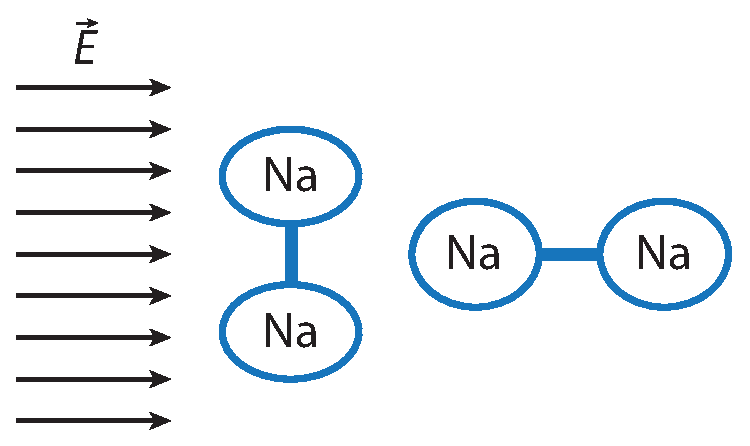
\includegraphics[width=1\textwidth]{Figures/dimerPolarizability.eps}
\caption[Alkali dimers in an electric field.]{\label{dimerOrientationFig}Two unique orientations of an alkali dimer with respect to the incident field. These two orientations have different polarizabilities, and thus different phase shifts in our atom interferometer.}
\end{figure}

%\begin{figure}
%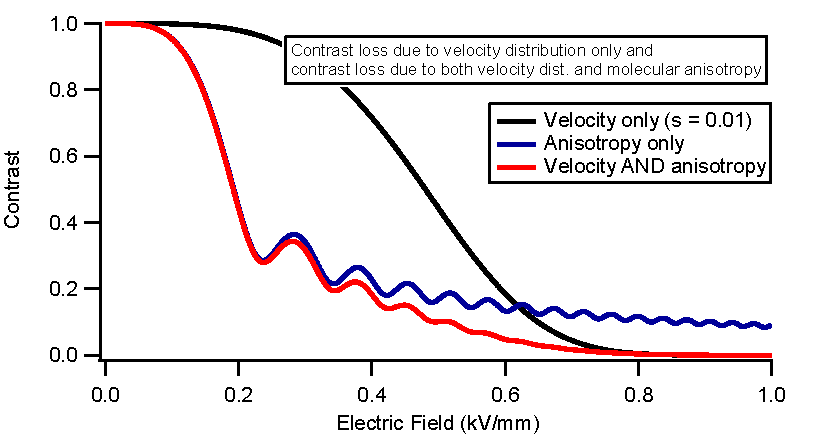
\includegraphics[width=1\textwidth]{Figures/molConVelAndGamma.pdf}
%\caption[Interferometer contrast loss due to the tensor polarizability of alkali dimers.]{\label{molConVelGammaBrief}Contrast loss due to anisotropy, velocity distribution, and both mechanisms combined. A measurement of the contrast loss signal may allow us to determine the polarizability anisotropy.}
%\end{figure}









